\section{System Implementation Plan}
\hspace*{0.7in} There are many important phases for implementation. Following are important phases and tasks of implementation: \\
The main phase is to study existing related application. All the necessary software for implementing the system must be installed on machine where the system is to be implemented. \\
\hspace*{0.7in} Software project management begins with set of activities that are collectively called project planning. Before the project can begins the team must estimate the work to be done, the resources that will be requiring, and the time that will elapse from start to finish. Planning involves estimation your attempt to determine how much money, how much effort, how many resource and how much time it will take to build to specific software base to system or product. \\
\hspace*{0.7in} Would one build a house without knowing how much you were about to spend for construction? Of course not and since most computer based system and products cost considerably more to build than a large house, it would seems reasonable to develop and estimate before you start creating a software.

\newpage
\begin{itemize}
  \item Project Plan for semester I and II:
\end{itemize}

\begin{table}[h]
\begin{center}
\caption{Project Plan for Semester I and II}\label{Project Plan for Semester I}
\begin{tabular}{|c|p{5cm}|c|c|c|} \hline
Sr.No & Phase & Start Date & End Date & Status\\ \hline
1 & Topic Selection & 26 June 2013 & 1 July 2013 & Completed \\		\hline
2 & Introduction & 1 July 2013 & 20 July 2013 & Completed \\		\hline
3 & Literature Survey & 21 July 2013 & 10 Aug 2013 & Completed \\		\hline
4 & System Requirement Specification & 11 Aug 2013 & 31 Aug 2013 & Completed \\		\hline
5 & System Design & 1 Sept 2013 & 7 Sept 2013 & Completed \\		\hline
6 & Technical Specification & 8 Sept 2013 & 21 Sept 2013 & Completed \\		\hline
7 & Project Estimate, Schedule, Team Structure & 22 Sept 2013 & 28 Sept 2013 & Completed \\		\hline
8 & Software Implementation & 29 Sept 2013 & 25 Apr 2014 & Completed  \\ \hline
9 & Software Testing & 1 Jan 2014 & 15 Feb 2014 & Completed  \\ \hline
10 & Experimental Results And Discussion & 16 Feb 2014 & 5 Apr 2014 & Completed \\ \hline
11 & Conclusion And Future Scope & 4 Apr 2014 & 5 Apr 2014 & Completed \\ \hline
 \end{tabular}
\end{center}
\end{table}


\subsection{Major Task}
$ \bullet $ Major task 1: \\
Provide overall planning and coordination for the implementation: \\
\hspace*{0.7in} This task refers to plan for the system implementation. It also provides the guideline for implementing the system. The tasks which are planned must be completed within date specified in  schedule. This will lead to successful completion of the project. \\
\\
$ \bullet $ Major task 2: \\
Provide appropriate training for personnel: \\
\hspace*{0.7in} This task refers to the training of the system developer on java,html and android framework. For successful completion of the scheduled task in estimated time, this is required. \\
\\
$ \bullet $ Major task 3: \\
Provide all needed technical assistance: \\
\hspace*{0.7in} The technical assistance must be provided whenever the work gets halt due to technical barriers.

\begin{table}[h]
\begin{center}
  \centering
  \caption{Major Task}\label{Major Task}
  \begin{tabular}{|c|c|c|} \hline
    \hline
    % after \\: \hline or \cline{col1-col2} \cline{col3-col4} ...
    Phase & Task & Description \\ \hline
    Phase1 & Requirement & Gather all the information for the selected topic. \\ \hline
    Phase2 & Analysis & Analyze all information on selected topic. \\ \hline
    Phase3 & Design & Assign the module. \\ \hline
  \end{tabular}
\end{center}
\end{table}


\subsection{Description of Implementation}
\hspace*{0.7in} For the implementation purpose the machine on which the system to be implemented, the Operating System must be Windows. For the implementation purpose developer will require Java knowledge as well aw HTML and Android SDK's knowledge. The implementation must be carried out in phases as described above. But the implementation can go Prototype wise development. One by one prototype must be implemented and further the functionalities must be implemented into that prototype without affecting previous prototype.

\subsection{Points-of-Contact}
\begin{table}[h]
\begin{flushleft}
\caption{Points-of-Contact}\label{Points-of-Contact}
\begin{tabular}{|c|c|c|} \hline
Role&	Name&	Contact Number\\ \hline
Project/Program Manager & Sushank Dahiwadkar& 9730971651, \\
& Anjali Kapadni & 9422499677 \\\hline		
System Developer or System Maintainer & Sushank Dahiwadkar, & 9730971651, \\
& Anjali Kapadni & 9422499677, \\ \hline	
Quality Assurance Manager & Sushank Dahiwadkar, & 9730971651, \\
& Anjali Kapadni & 9422499677, \\ \hline	
Database Administrator& Sushank Dahiwadkar& 9730971651, \\ \hline

\end{tabular}
\end{flushleft}
\end{table}

\subsection{Security and Privacy}
\hspace*{0.7in} For performing operations with NoSQL KVstore user need to Connect with KVClient for that user need to provide Store Name, Port Number and Host Name to logged into UI to perform these operations.
If user is not able to connect to store then he/she may not be able to perform tha operations.

\section{Project Scheduling}
\hspace*{0.7in} Project scheduling is the process of putting together a time line for all the activities in the project. This involves examining the interdependencies of all of the activities, and coordinating all the tasks to ensure a smooth transition from the beginning to the end of the project. There are many different methods of scheduling, which can address the requirements of the type of project resulting in different pictorial representations of the schedules. For example use Gantt charts to represent the project scheduling. \\
\\ \\
$ \bullet $ Gantt Chart of Scheduling for Semester I is as follows : \\
\begin{figure}[h]
\centering
  % Requires \usepackage{graphicx}
  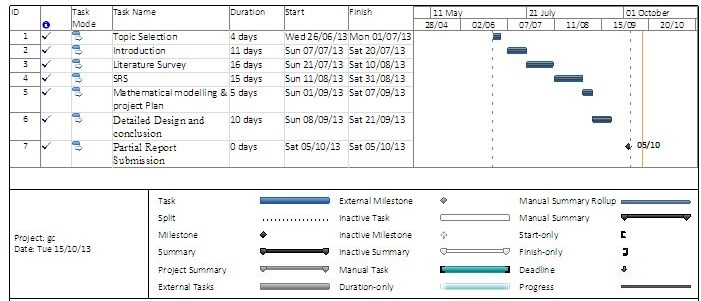
\includegraphics[width=17cm,height=13cm]{fig34.png}
  \caption{Gantt Chart of Scheduling of Sem I}\label{Gantt Chart of Scheduling Sem I}
\end{figure}

\newpage
$ \bullet $ Gantt Chart of Scheduling for Semester II is as follows : \\
\begin{figure}[h]
\centering
  % Requires \usepackage{graphicx}
  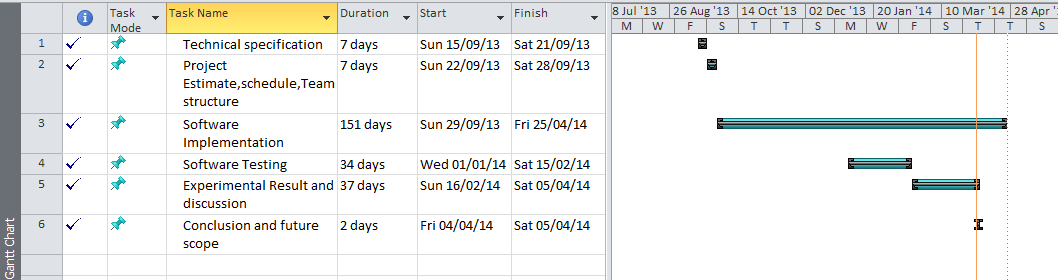
\includegraphics[width=14cm,height=7cm]{fig34-1.png}
  \caption{Gantt Chart of Scheduling Sem II}\label{Gantt Chart of Scheduling Sem II}
\end{figure}

\section{Feasibility Study}
\subsection{COCOMO Model}
Constructive cost model is one of the most widely used and discussed software cost estimation model. The Query by example based Video Retrieval System uses COCOMO MODEL. The basic COCOMO MODEL computes software development efforts and cost as a function of program size express in estimated line of code.

\begin{table}[h]
\begin{flushleft}
\centering
\caption{Analysis and Estimation Cocomo model} \label{Analysis and Estimation Cocomo model}
\begin{tabular}{|c|p{2cm}|p{2cm}|p{2cm}|p{2cm}|} \hline
Software Project & $a_{b}$ & $b_{b}$ & $c_{b}$ & $d_{b}$ \\ \hline
 \textbf{Organic} & 2.4 & 1.05 & 2.5 & 0.38 \\ \hline
 Semi Detached & 3.0 & 1.12 & 2.5 & 0.35 \\ \hline
 Embedded & 3.6 & 1.20 & 2.5 & 0.32 \\ \hline
 \end{tabular}
 \end{flushleft}
 \end{table}

\textbf{"A Tool for Managing Key Values pair on Oracle NoSQL Database"} is an \emph{Organic} project. \\

\hspace*{0.7in} $\maltese$  Effort = $a_{b}KLOC^{b_{b}} $ \\
\hspace*{0.7in} $\maltese$  Duration = $ c_{b}KLOC^{d_{b}} $ \\

\begin{table}[h]
\begin{flushleft}
\centering
\caption{Calculation} \label{Calculation}
\begin{tabular}{|c|c|} \hline
Functions (Modules) & Estimated LOC  \\ \hline
Module 1 (Connection) & 60 \\ \hline
Module 2 (Operation Selection) & 1000 \\ \hline
Module 3 (Result) & 700 \\ \hline
Total & 1760 \\ \hline
 \end{tabular}
 \end{flushleft}
 \end{table}

 \begin{itemize}
   \item $a_{b}=2.4$
   \item $b_{b}=1.05$
   \item $c_{b}=2.5$
   \item $d_{b}=0.38$
   \item KLOC=1.76
\end{itemize}

$\maltese$  Effort = $a_{b}KLOC^{b_{b}}$ \\
\hspace*{0.10in} = 2.4 * $(1.76^{1.05})$ \\
\hspace*{0.10in} = 4.345 persons/month. \\
\\
$\maltese$  Duration  = $c_{b}KLOC^{d_{b}} $ \\
\hspace*{0.10in} = 2.5 * $(1.76^{0.38})$ \\
\hspace*{0.10in} = 3.1 months \\
\\
$\maltese$  Number  of  people recommended  = $\frac{Efforts}{Duration}$ \\
\hspace*{0.10in} = $\frac{4.345}{3.1}$ \\
\hspace*{0.10in} = 1.5 persons \\
\hspace*{0.10in} = $\sim$ 2 person \\
\\
\textbf{LOC based Estimation:} \\
\hspace*{0.5in} $ \diamond $ The average productivity for our product is : 600 LOC/Month \\
\hspace*{0.5in} $ \diamond $ The labour rate estimated is : Rs. 1000/- per month \\
\hspace*{0.5in} $ \diamond $ The cost per line of code is : approximately Rs. 6 \\
\hspace*{0.5in} $ \diamond $ Base on LOC estimated and historical productivity data, \textbf{Total estimated project cost is : Rs. 22560/-}
\newpage
\section{Team Structure}
The team structure for this project is as follows :
\begin{figure}[h]
\centering
  % Requires \usepackage{graphicx}
  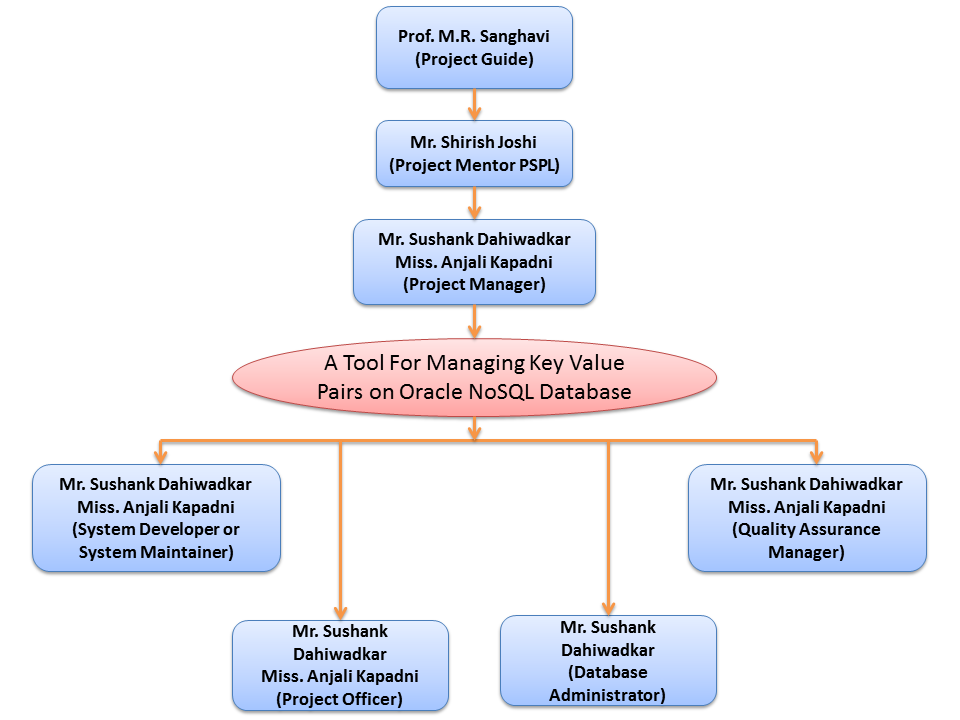
\includegraphics[width=15cm,height=15cm]{TS.png}\\
  \caption{Team Structure} \label{Team Structure}
\end{figure} 